\section{Results}

\subsection{Qualitative}

We drew on the NASSS framework to help understand the socio-technical factors likely to affect the adoption and scale-up of SAMueL-2 technology. Participants were hopeful the SAMueL-2 technology could address variance in thrombolysis practice. It was seen as particularly suitable for junior clinicians, non-stroke specialists and at district general hospitals and offered value for training, reviewing clinical cases, and quality improvement. We identified three learning  points  which  may  facilitate  further implementation of the technology:
\begin{itemize}

    \item Given reservations expressed about the underpinning SSNAP data, it is important to reassure intended adopters about the integrity of modelling based on this data.
    First, given reservations expressed by some of our participants and healthcare professionals elsewhere about the underpinning SSNAP data it seems important to ensure that intended adopters are reassured about the integrity of modelling based on this data.

    \item Evidence indicated that emergency department physicians may have less confidence in the evidence base for thrombolysis.
     Second, evidence from this research and elsewhere indicates that the ED physicians’ may have less confidence in the evidence base for, and safety of thrombolysis. It is therefore likely that more work will need to be done with the ED physician community to build trust in the SAMuel-2 technology: recruiting ED physicians as brokers/clinical champions may help to address this. 
    
    \item Perceived lack of funding and stroke workforce shortages may impede quality improvement and adoption of new technologies such as SAMueL-2.
    Third, perceived lack of funding/resource and stroke workforce shortages may impede quality improvement and adoption of new technologies such as SAMueL-2. It will therefore be vital to address these concerns to ensure sustained use and adoption

\end{itemize}

\subsection{Quantitative}

\subsubsection{Influences on best and worst outcomes across a patient cohort}

In order to understand general characteristics affecting outcomes, using the results from the multiclass classification model (ROC-AUC 0.796; 0.001 standard deviation across the 5 k-folds), we have shown how patient feature values, and stroke team attended, affected the likelihood of having the best (mRS 0) or worst (mRS 6) outcomes (figure \ref{fig:shap_outcome_model}) across the 15,680 test patients (which were not used to train the model). Feature values that contributed to the best outcome on discharge (mRS 0) were no prior disability, milder stroke, earlier thrombolysis, younger, no atrial fibrillation diagnosis, and precisely known stroke onset time. Feature values that contributed to the worst outcome on discharge (mRS 6) were higher prior disability, more severe stroke, later or no thrombolysis, older, diagnosis of atrial fibrillation, and an imprecisely known onset time. The hospital attended also affected outcome predictions, with a  larger contribution from the attended hospital contribution for mRS 0, rather than mRS 6, at discharge. 

\begin{figure}[ht]
    \centering
    \begin{subfigure}{.5\textwidth}
      \centering
      \captionsetup{width=.9\linewidth}
      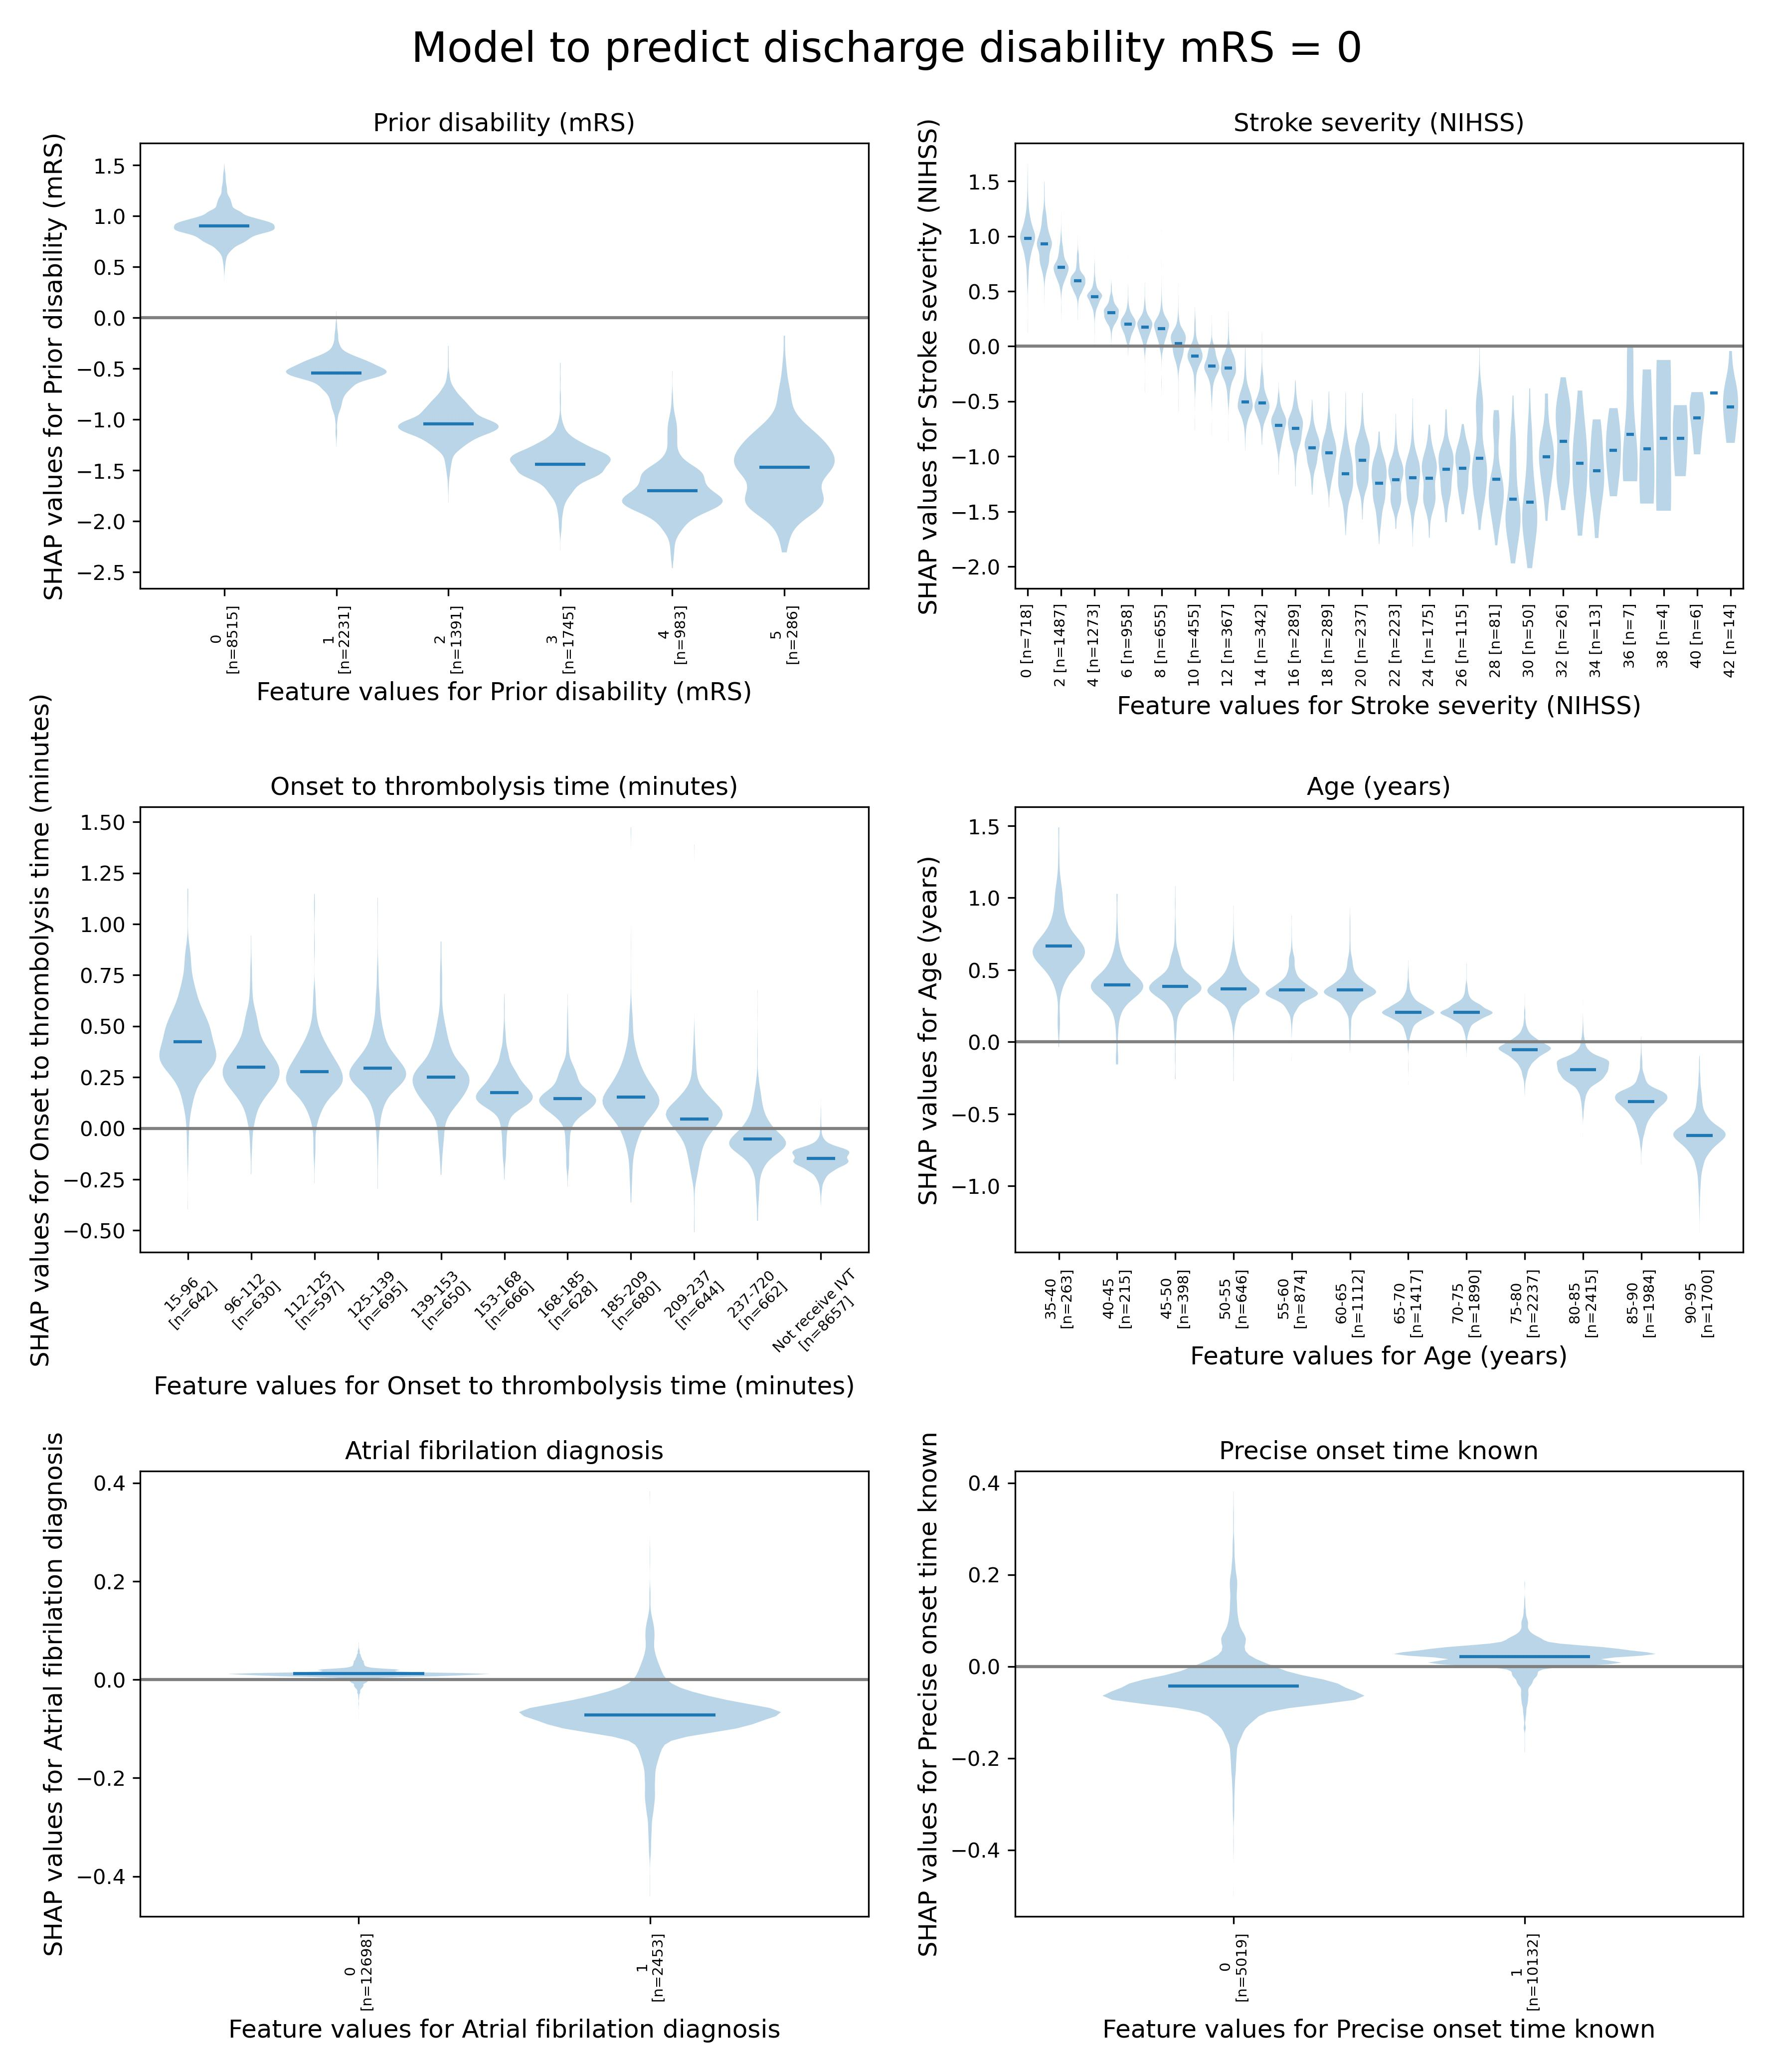
\includegraphics[trim={0 0 0 1.2cm}, clip, width=0.95\linewidth]      {./images/053_xgb_7_features_1fold_thrombolysis_shap_violin_all_features_for_mRS0}\\

    \end{subfigure}%ults
    \begin{subfigure}{.5\textwidth}
      \centering
      \captionsetup{width=.9\linewidth}
      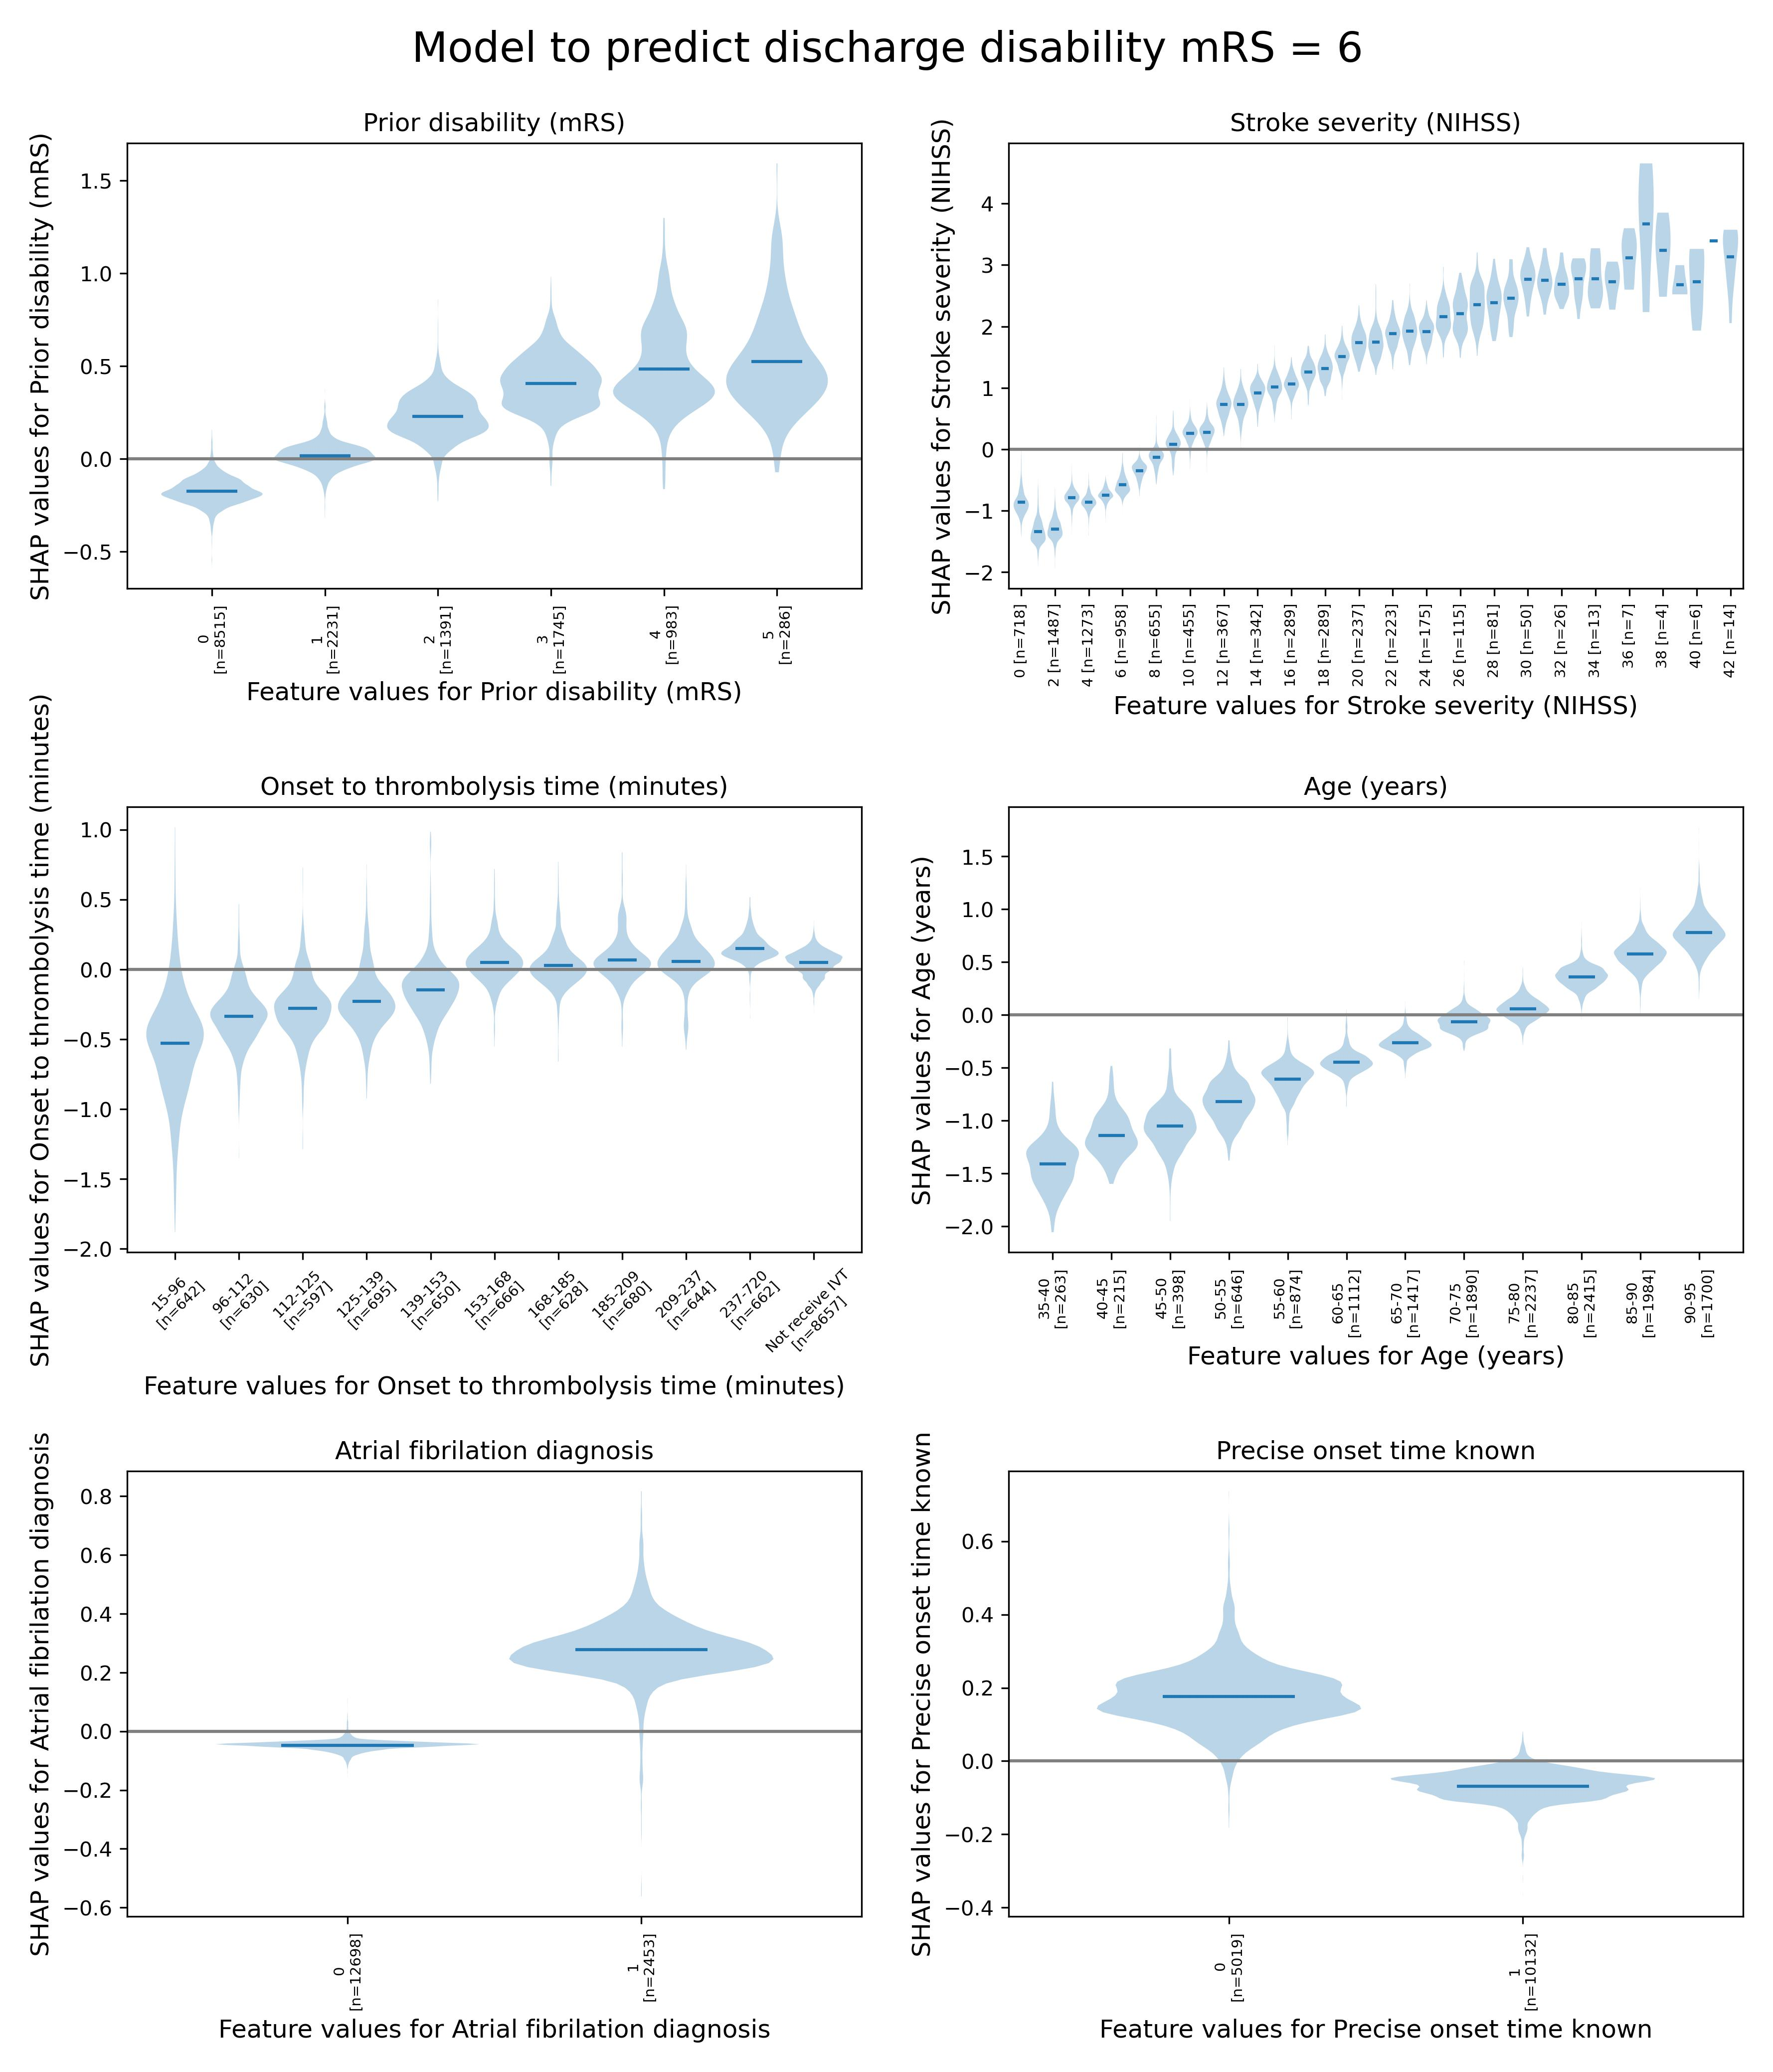
\includegraphics[trim={0 0 0 1.2cm}, clip, width=0.95\linewidth]      {./images/053_xgb_7_features_1fold_thrombolysis_shap_violin_all_features_for_mRS6}\\
    \end{subfigure}
    \hfill
    \begin{subfigure}{.5\textwidth}
      \centering
      \captionsetup{width=.9\linewidth}
      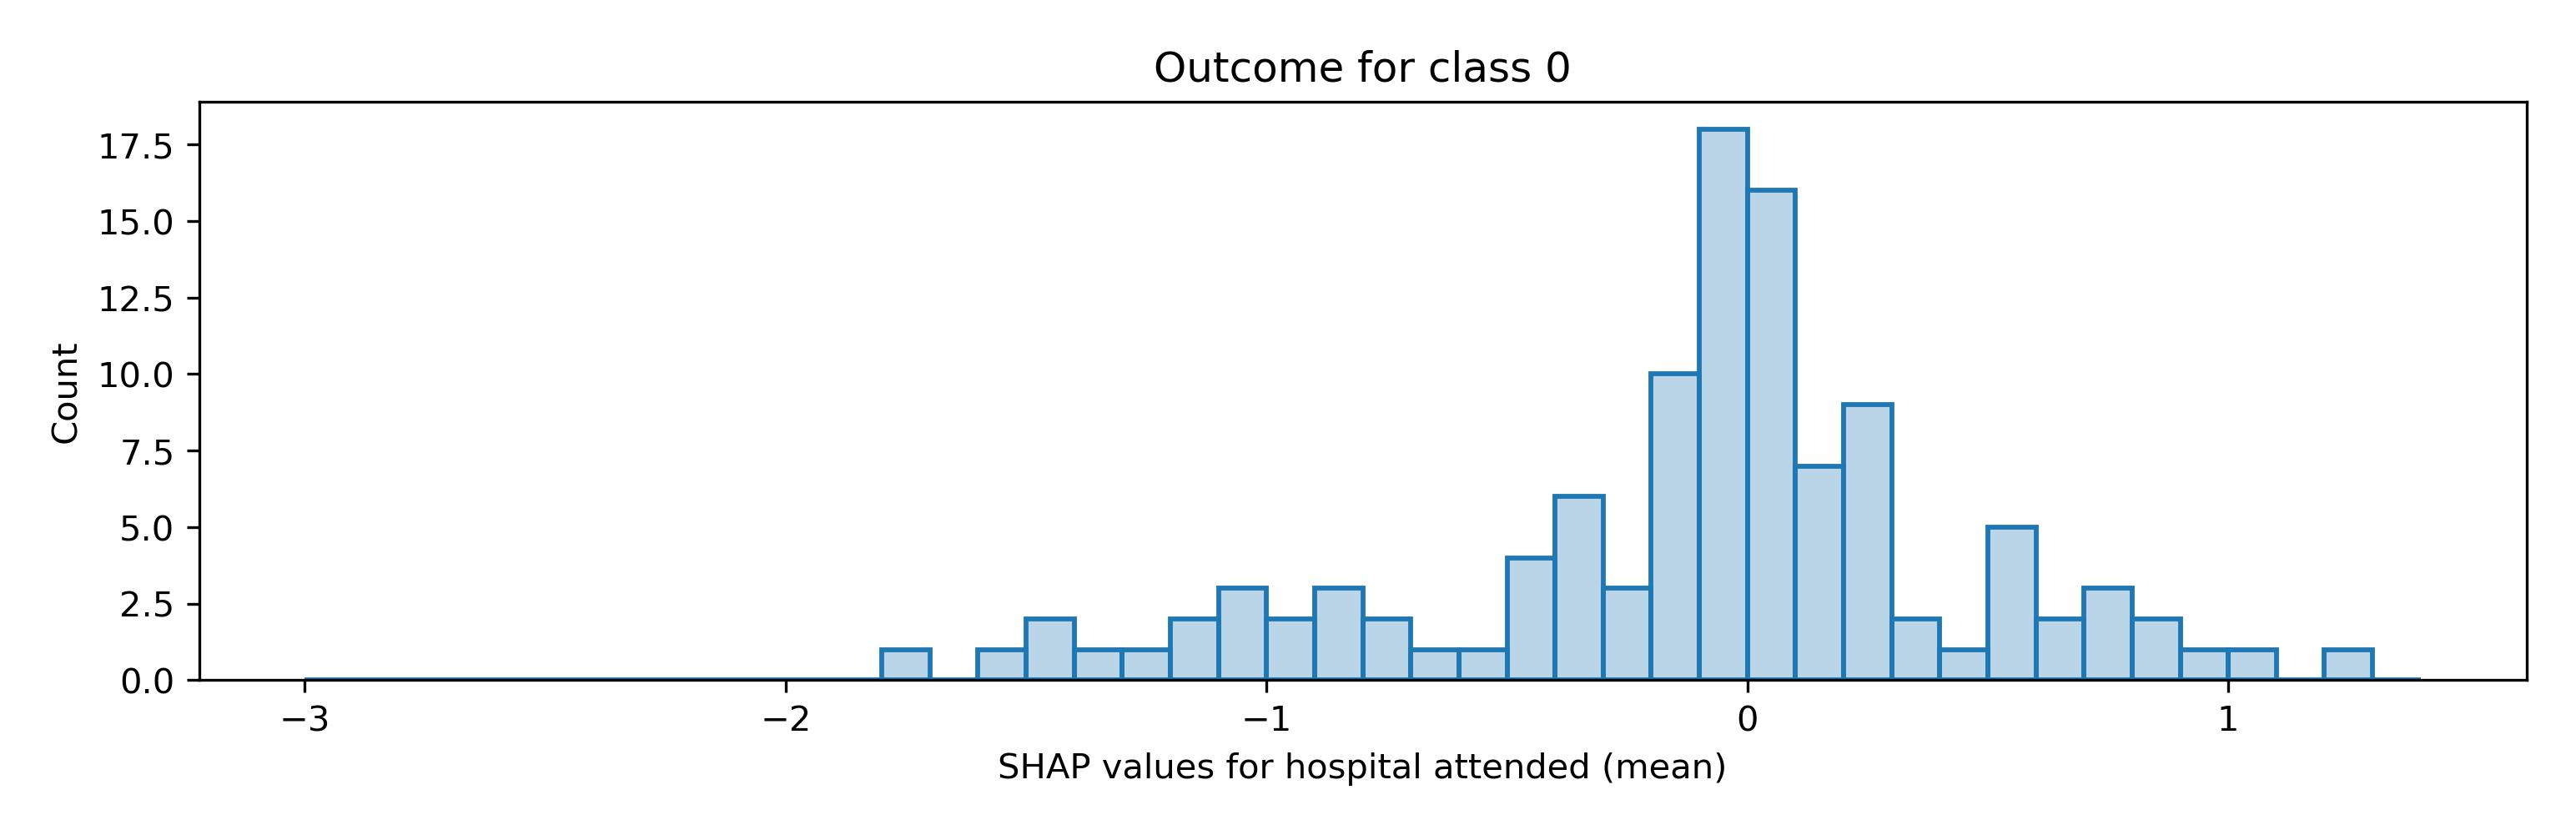
\includegraphics[trim={0 0 0 1cm}, clip, width=1\linewidth]    {./images/053_xgb_7_features_1fold_hosp_shap_hist_mrs0}\\
      \caption{\footnotesize{SHAP values for the likelihood of no disability on discharge (mRS 0). Base SHAP value = -0.405}}
      \label{fig:mrs0_violin}
    \end{subfigure}%ults
    \begin{subfigure}{.5\textwidth}
      \centering
      \captionsetup{width=.9\linewidth}
      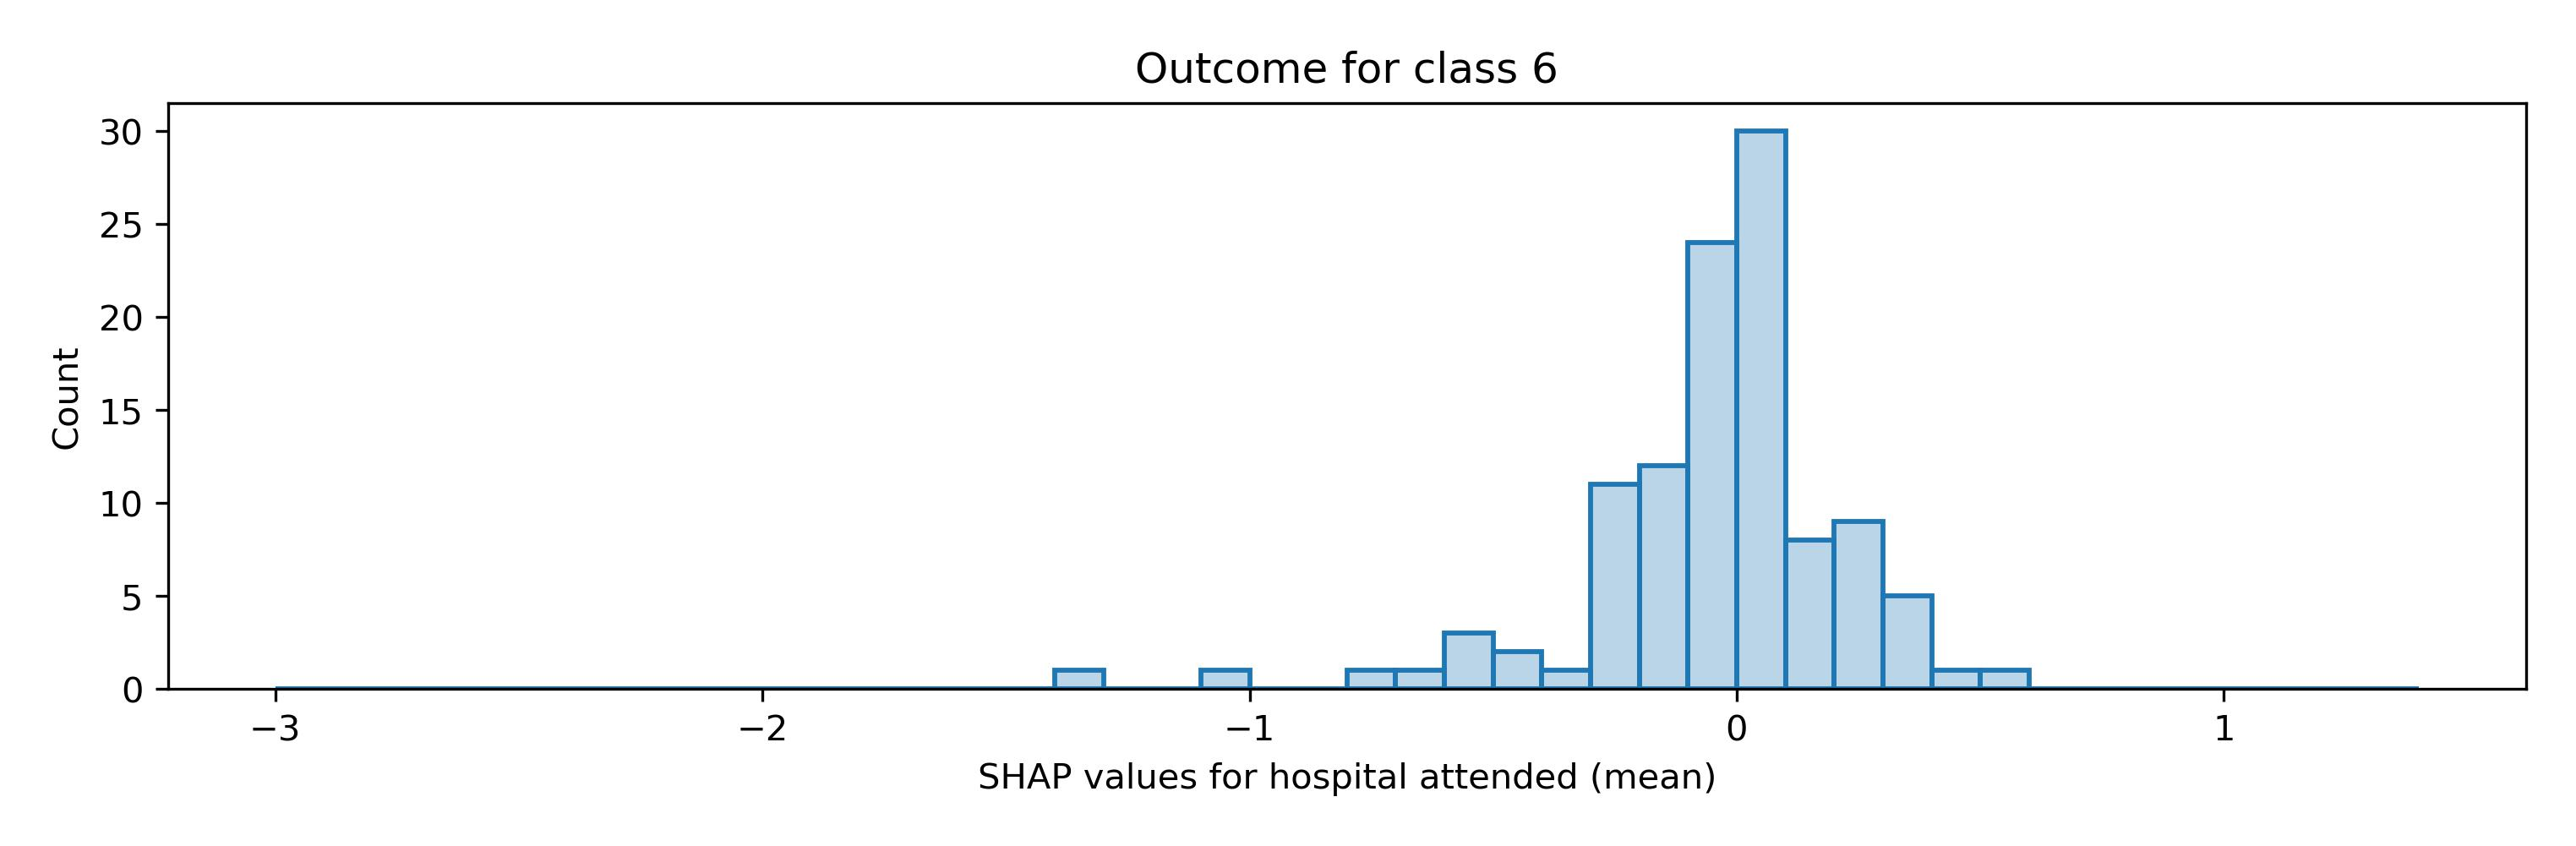
\includegraphics[trim={0 0 0 1cm}, clip, width=1\linewidth]
        {./images/053_xgb_7_features_1fold_hosp_shap_hist_mrs6}\\
      \caption{\footnotesize{SHAP values for the likelihood of death at discharge (mRS 6). Base SHAP value = -0.311}}
      \label{fig:mrs6_violin}
    \end{subfigure}
  \caption{Plots showing the relationship between SHAP values and feature values for best or worse possible outcomes. Left: Predicting the likelihood of having no disability at discharge (mRS 0). Right: Predicting the likelihood of being dead at discharge (mRS 6). Top: Violin plots showing the relationship between SHAP values and feature values. The horizontal line shows the median SHAP value. Bottom: Histogram showing the frequency of the mean SHAP value for the hospital attended.}
    \label{fig:shap_outcome_model}
\end{figure}

\subsubsection{Are the results from the thrombolysis clinical trial meta-analysis seen in real life outcomes?} 

The overall accuracy ranged from 77.6\% to 89.7\% across the six \textit{thrombolysis outcome mRS threshold} models (standard deviation across the 5 k-folds ranged from 0.001 to 0.002) \cite{pearn_thrombolysis_2024}. Receiver Operating Characteristic Area Under Curve (ROC-AUC) ranged from 0.852 to 0.893 across the six models (standard deviation across the 5 k-folds ranged from 0.001 to 0.002). Thrombolysis was found to be associated with a statistically significant improvement in the odds of having a good outcome using any mRS threshold. Regression analysis predicted a maximum 2.5-fold improvement in odds of achieving mRS 0-1, with a decline to no treatment effect at 5 hours 28 minutes post-onset. The observed beneficial effect is very similar to Emberson’s meta-analysis \cite{emberson_effect_2014} of a maximum 2.0-fold improvement in odds of achieving mRS 0-1, with a decline to no treatment effect at 6 hours 18 minutes post-onset.

\begin{figure}[ht]
    \centering
    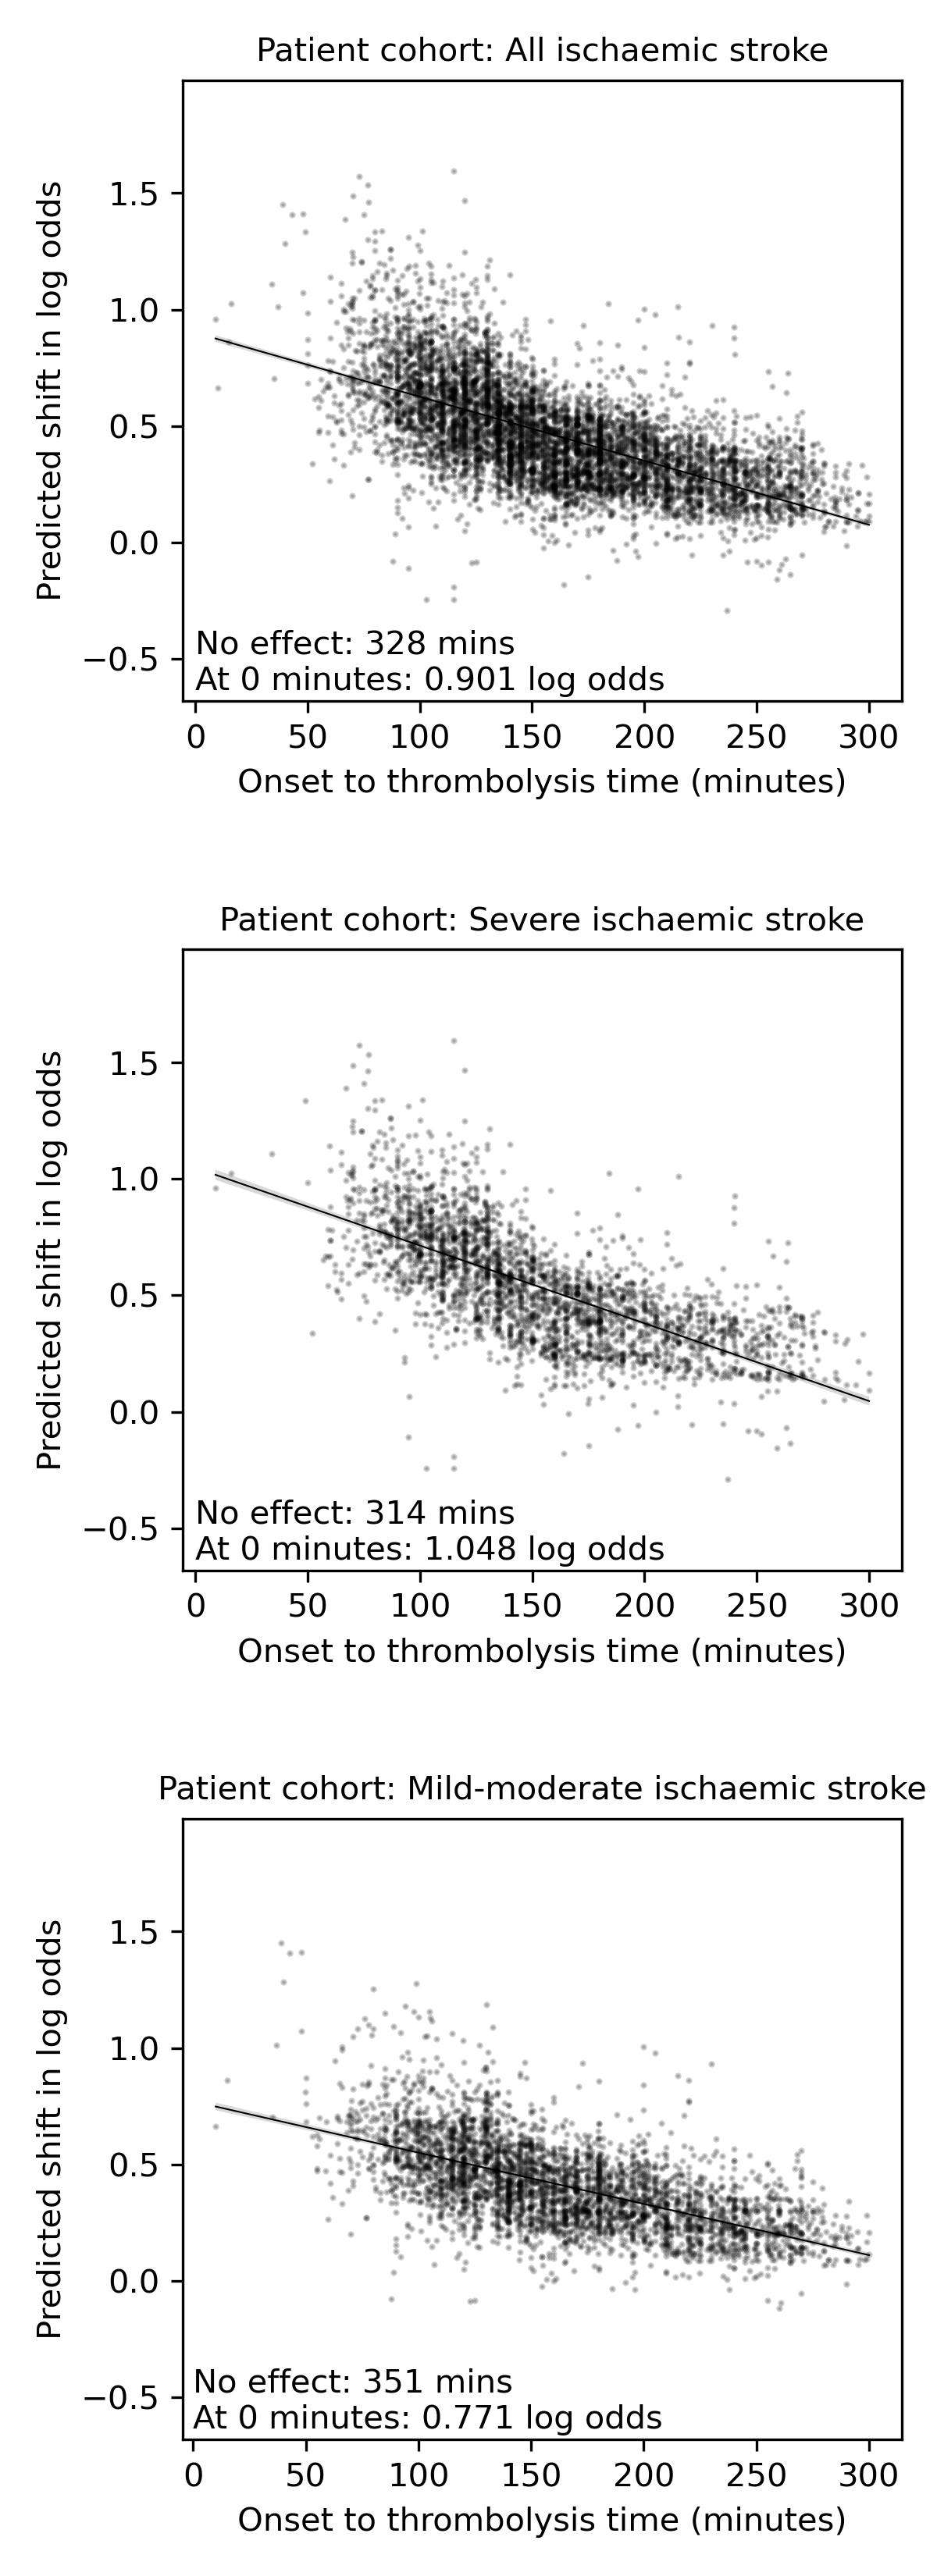
\includegraphics[width=0.40\textwidth]{./images/p3_regression_v1}\\
    \caption{A linear regression fit to the contribution from receiving thrombolysis in having a good outcome (mRS 0-1) at discharge, with respect to the onset to thrombolysis time (for patients treated within 300 minutes). Top: all treated stroke patients (n = 6,796); Middle: treated severe stroke patients, NIHSS 11+ (n = 2,856); Bottom: treated mild-moderate stroke patients, NIHSS 0-10 (n = 3,940).}
    \label{fig:linear_regression_plots}
\end{figure}

\newpage
\begin{table}[H]
    \caption{Fitting linear regression to the shift in the contribution from receiving thrombolysis towards having a good outcome (mRS 0-1) at discharge with respect to the onset to thrombolysis (OTT) time. Linear regression statistics for different patient cohorts. We used NIHSS 0-10 to define mild-moderate strokes, and NIHSS 11+ to define severe strokes.}
    \centering
        \begin{tabular}{lllllllll}
        \toprule
         Ischaemic stroke type & Variables & coef & std err & t & P$>$$|$t$|$ & [0.025 & 0.975] \\ 
         \midrule
        All & Constant & 0.9012 & 0.007 & 132.519 & 0.000 & 0.888 & 0.915\\
        & OTT time (min) &  -0.0027  & 4.04e-05 & -68.058 & 0.000 & -0.003 & -0.003\\   
        \midrule
        Severe & Constant & 1.0476  &    0.011  & 96.746 & 0.000 & 1.026 & 1.069\\
        & OTT (mins) & -0.0033 &  6.67e-05  & -50.042 & 0.000 & -0.003 & -0.003\\ 
        \midrule
        Mild-moderate & Constant &           0.7708 &     0.008   & 97.613 & 0.000 & 0.755 & 0.786\\
        & OTT time (mins) &  -0.0022 &   4.57e-05 & -48.109 & 0.000 & -0.002 & -0.002\\
        \bottomrule
        \end{tabular}
      \label{fig:stats_table_mrs1}
\end{table}


\subsubsection{Are the patients who would benefit from thrombolysis the same ones as those receiving it? \cite{pearn_are_2024}}

44\% of the study population received thrombolysis. Taking a better outcome with treatment to be defined as both a better average disability likelihood and a reduction in probability of being mRS 5-6, overall, 60\% of patients in the study population were predicted to benefit from thrombolysis. Of those who did receive thrombolysis, 73\% were predicted to have a better outcome with treatment. Of those who did not receive thrombolysis, 49\% were predicted to have a better outcome with treatment. Figure \ref{fig:decriptive_plots_2_cohorts} shows the distribution of feature values for the two patient cohorts: (i) those that received thrombolysis but were predicted to not have a better outcome with thrombolysis, (ii) those that did not receive thrombolysis but were predicted to have a better outcome with thrombolysis. When examining individual feature values in this way we did not identify any features that could be used in isolation to identify those patients who would benefit from thrombolysis but did not receive thrombolysis (or vice-versa).

\begin{figure}
    \centering
    \captionsetup{width=1\linewidth}
    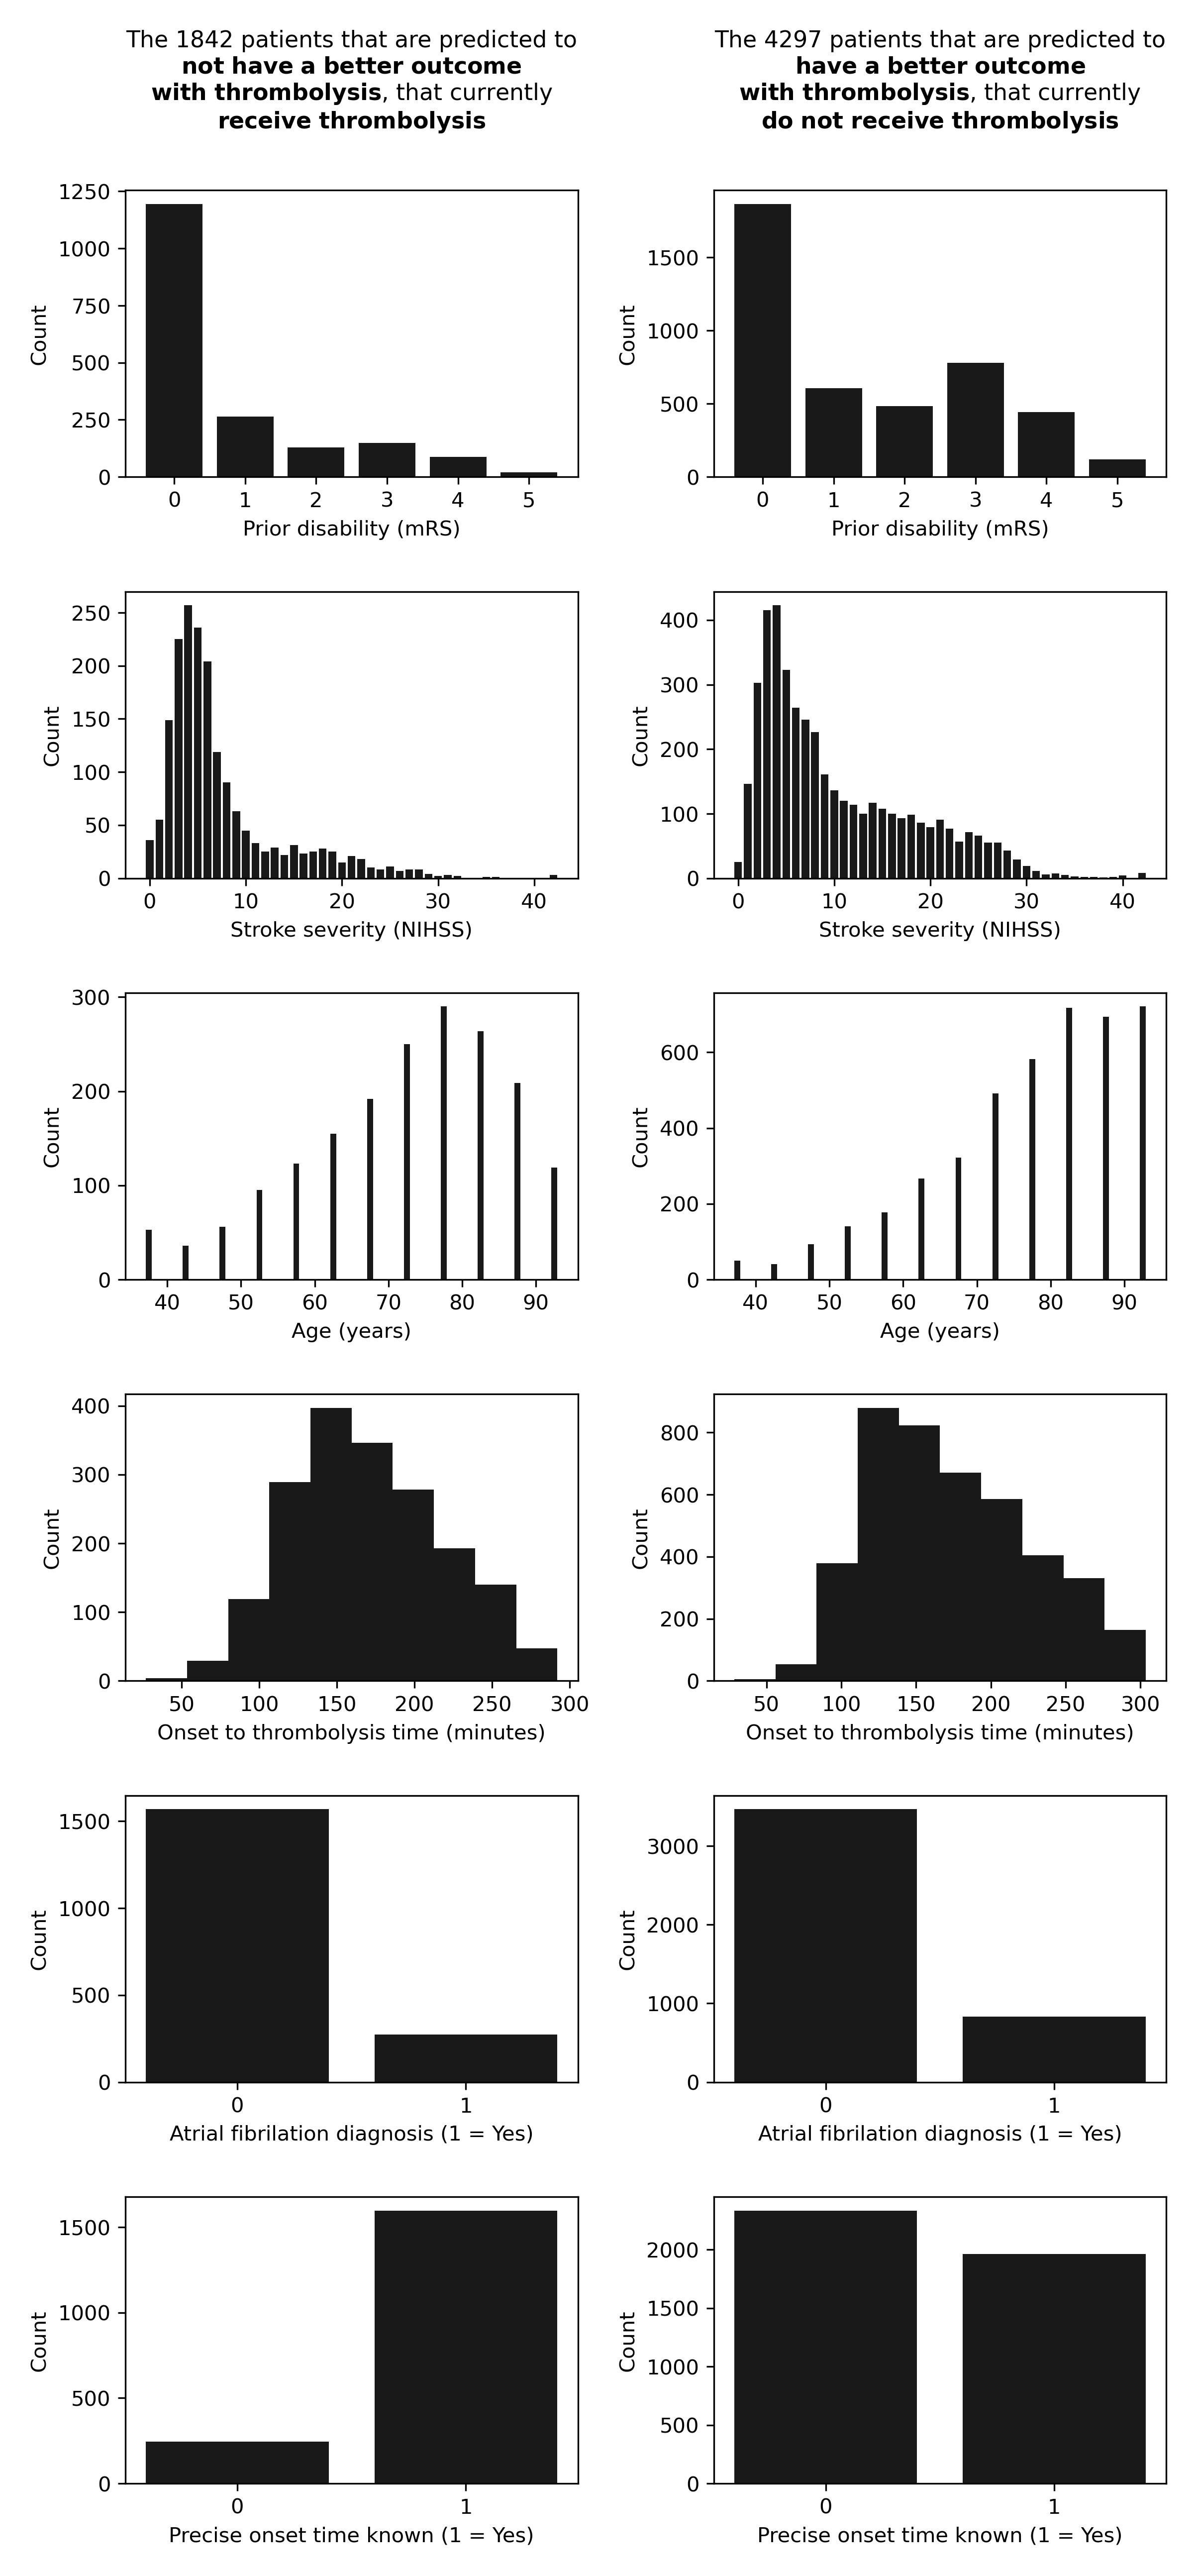
\includegraphics[width=0.6\linewidth]{./images/210_xgb_all_data_multiclass_outcome_descriptive_plots_2_patient_cohorts}\\
  \caption{Plots showing the frequency of feature values for patient cohorts where actual treatment decision differed from best predicted outcome. \textit{Left}: patients that were predicted to not have a better outcome with thrombolysis, but received thrombolysis. \textit{Right}: patients that were predicted to have a better outcome with thrombolysis, but did not receive thrombolysis.}
  \label{fig:decriptive_plots_2_cohorts}
\end{figure}


\subsubsection{Hospital trade-off between maximising benefit from thrombolysis and minimising risk of harm from thrombolysis}

The XGBoost \textit{thrombolysis decision} model had an accuracy of 78.7\% and ROC-AUC of 0.86. Figure \ref{fig:hosp_shap_scatter} shows the trade-off between the individuals hospital sensitivity and specificity towards giving treatment. We found that those hospitals attaining a higher predicted \textit{sensitivity} of treatment (not missing patients who would benefit from treatment) also tended to have a lower \textit{specificity} (giving thrombolysis to patients who would likely not benefit from it).

\begin{figure}
    \centering
    {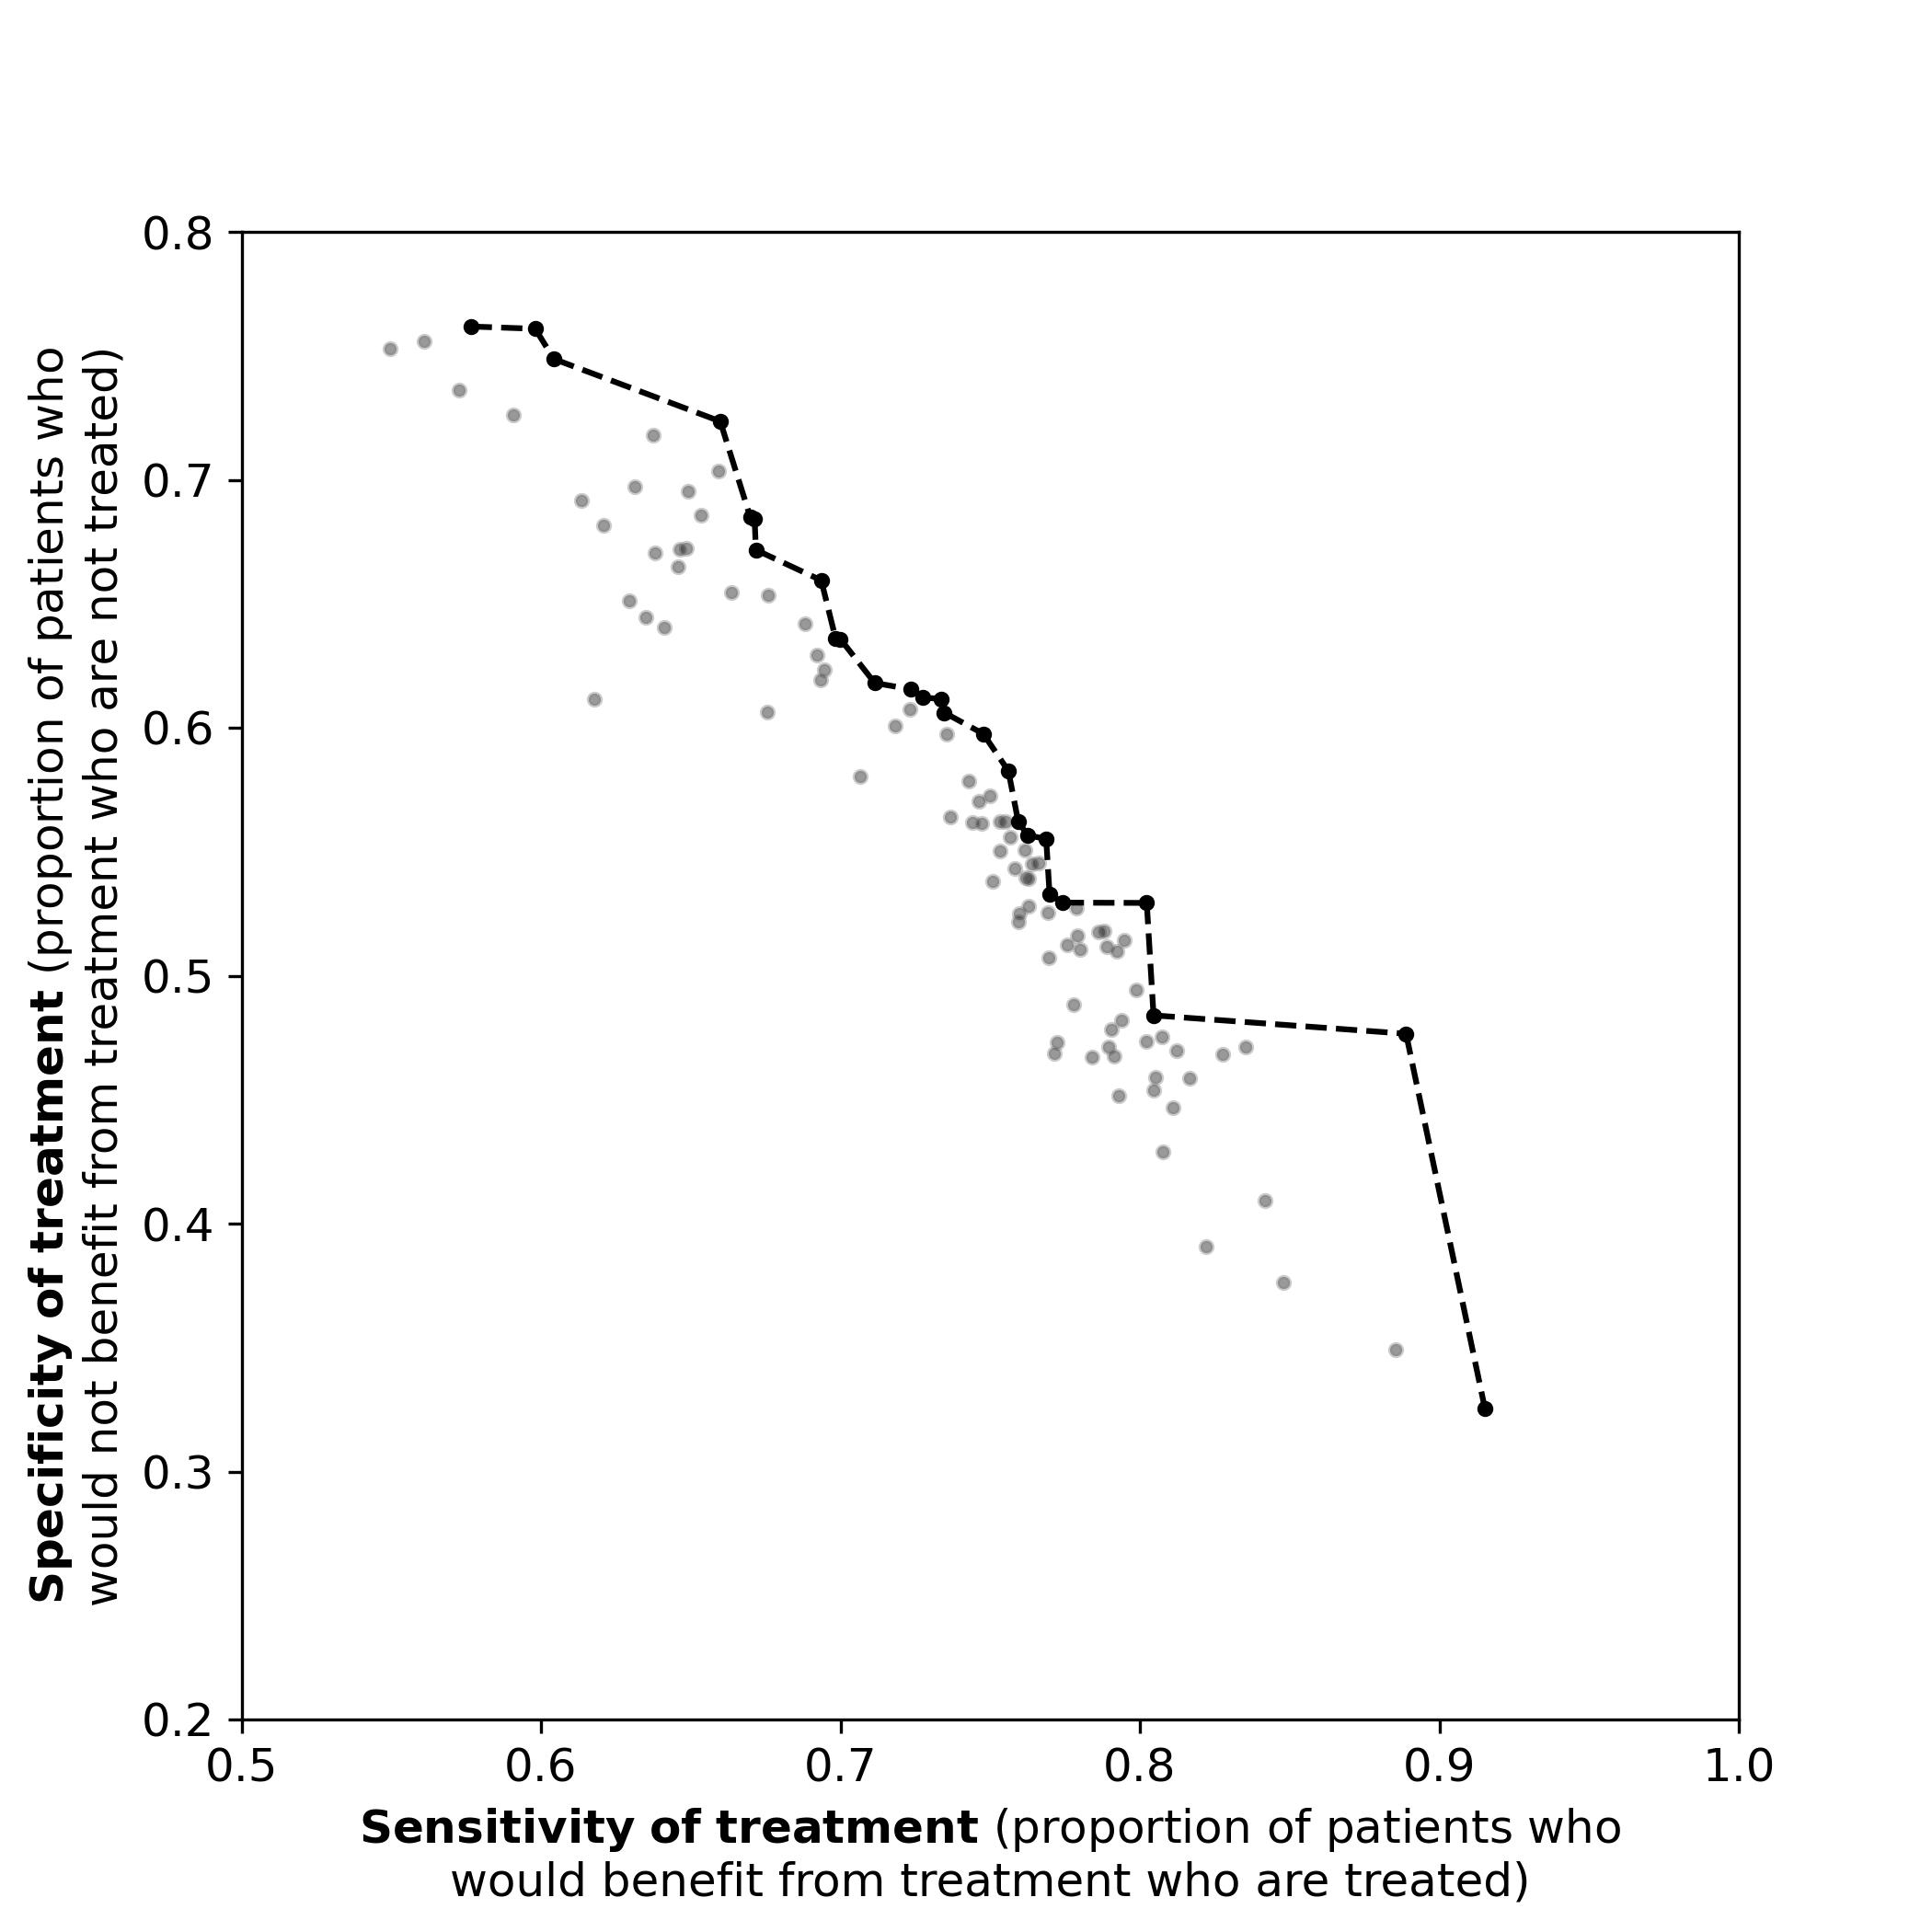
\includegraphics[width=0.65\linewidth]{./images/p4_spec_sens}} 
    \caption{\textit{Sensitivity} (proportion of patients who were predicted to benefit from thrombolysis who were predicted to receive thrombolysis) and \textit{specificity} (proportion of patients who were predicted \textit{not} to benefit from thrombolysis who were predicted \textit{not} to receive thrombolysis) for each stroke team. The dotted line shows the hospitals on the Pareto front where there are no hospitals that have a better \textit{sensitivity} without a worse \textit{specificity}, or vice-versa.}
    \label{fig:hosp_shap_scatter}
\end{figure}

\subsubsection{Comparing decision-making across stroke teams}

The XGBoost \textit{thrombolysis decision} model had an accuracy of 78.7\% and ROC-AUC of 0.86, and the XGBoost \textit{thrombolysis outcome multiclass} model had an accuracy of 78.7\% and ROC-AUC of 0.86. Prototype patients revealed variation in likely decisions between stroke teams (figure \ref{fig:thrombolysis_rates_prototype_patients1}). While almost all stroke teams would give thrombolysis to the \textit{ideal} candidate for thrombolysis, the predicted use of thrombolysis varied more as one characteristic was changed from the \textit{ideal} candidate. In particular there was a very wide range in likelihood of a patient with a mild stroke (NIHSS 3) receiving thrombolysis. Mild stroke (NIHSS 0-4) represents a large proportion of admissions (54\% of all emergency stroke admissions, and 38\% of ischaemic stroke patients arriving by ambulance within 4 hours of known stroke onset). Combinations of \textit{non-ideal} patient characteristics reduced predicted use of thrombolysis further (again with significant variation between stroke teams), especially when the non-ideal characteristic was a mild stroke.

\begin{figure}
    \centering
    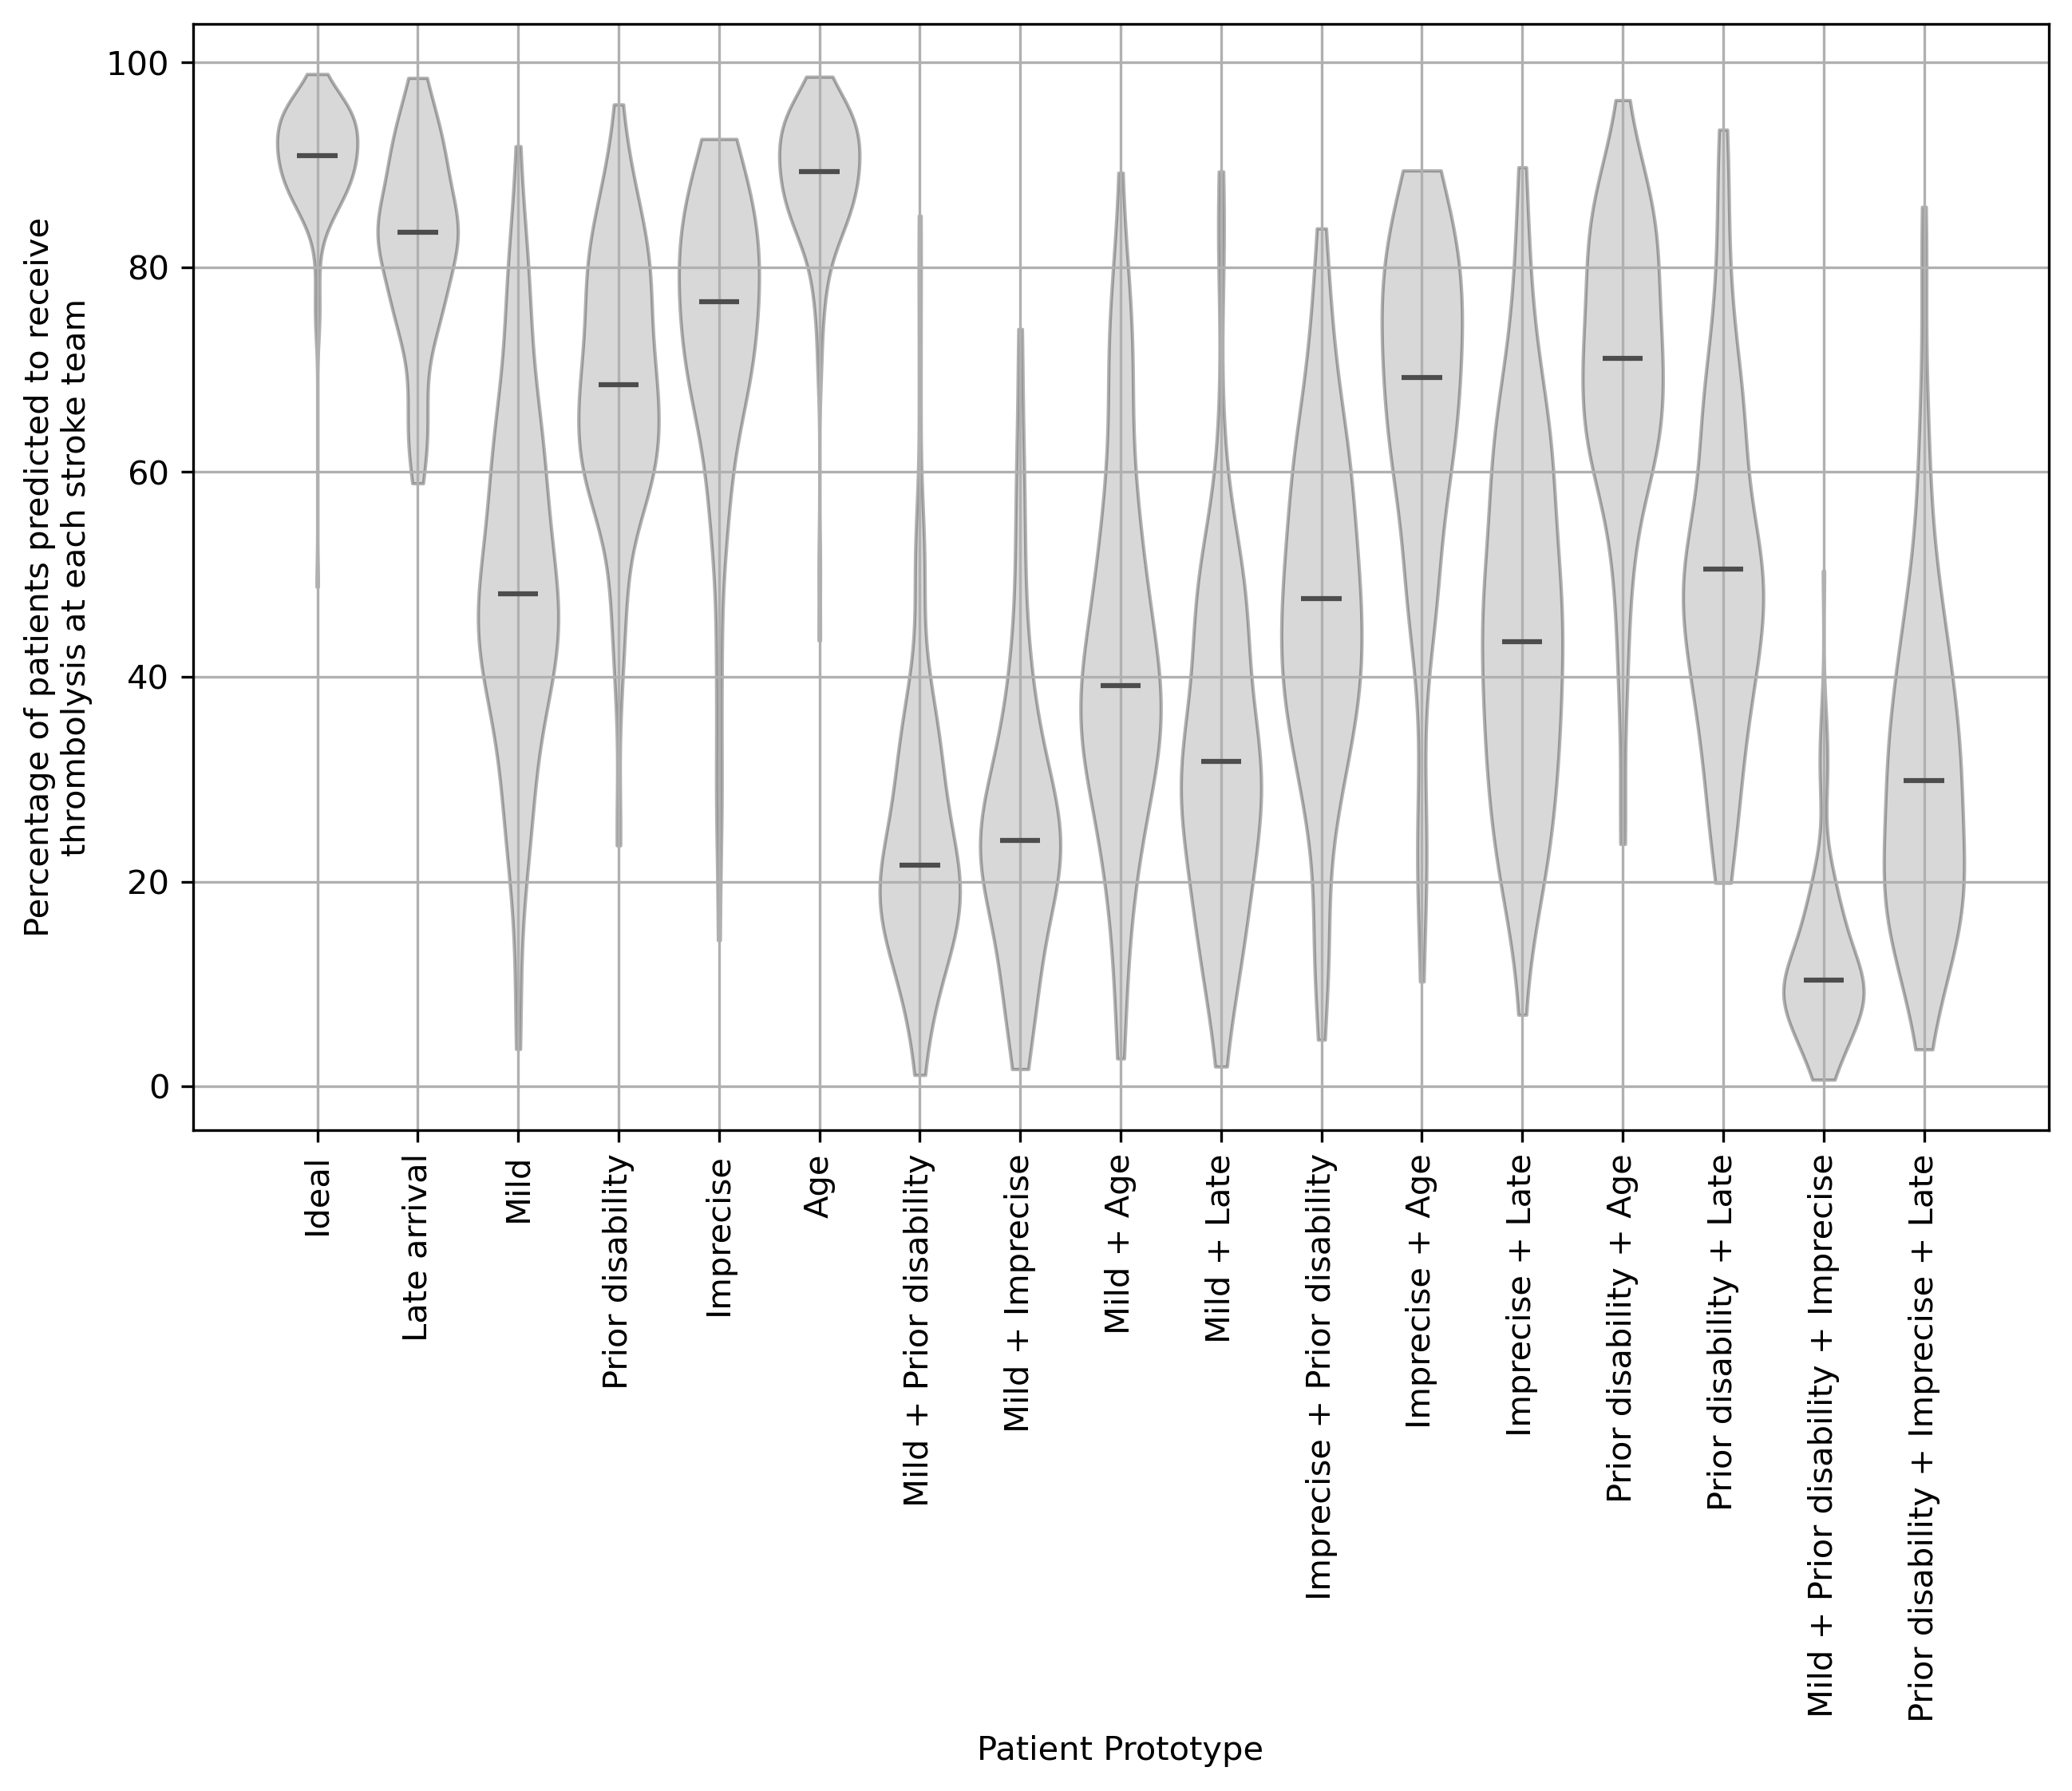
\includegraphics[width=0.75\linewidth]{images/p5_prototype_decision.png}
    \caption{Violin plots showing the variation in predicted thrombolysis rates for 17 patient prototypes across stroke teams. \textit{Ideal}: onset-to-arrival = 90 minutes; arrival-to-scan = 15 minutes; onset-to-thrombolysis = 120 minutes; stroke severity (NIHSS) = 15; pre-stroke disability (mRS) = 0; age = 72.5; precisely known onset; onset not during sleep; stroke type = infarction; patient has no atrial fibrillation and is not receiving anticoagulants for atrial fibrillation; \textit{Late arrival}: as \textit{ideal} but onset-to-arrival = 225 minutes and onset-to-thrombolysis = 255 minutes; \textit{Mild}: As \textit{ideal} but stroke severity = 3; \textit{Prior disability}: as \textit{ideal} but pre-stroke disability = 3; \textit{Imprecise}: as \textit{ideal} but stroke onset time estimated; \textit{Age}: as \textit{ideal} but age = 87.5.}
    \label{fig:thrombolysis_rates_prototype_patients1}
\end{figure}